% Technology assumptions of the Catalyst model: justification document.
%
% Pages 1 and 2 hold the two tables generated from ../technology_assumptions.csv (build/table.tex,
% rule assumptions_table); every technology name in them is a hyperlink (\techlink below) to
% \label{sec:<technology>} in that technology's subsection, where the sources and derivations
% of the row (the CSV's comment and source columns) are argued in prose. Each subsection title
% carries the CAPEX typed by hand -- deliberately not wired from the CSV, so that text and
% table drift apart visibly when one is changed without the other (build_table.py warns, also
% for a missing label).
% Add text, figures (doc/figures/) and references (references.bib) in doc/sections/*.tex.
%
% Build: snakemake -s ../assumptions.smk -c1 (from ..), or bash config-pypsa-earth/run.sh assumptions.
% Style after Way, Mealy & Farmer, INET Oxford WP 2021-01 (kpfonts, single column, booktabs, author-year).

\documentclass[11pt,a4paper]{article}
\usepackage[T1]{fontenc}
\usepackage[utf8]{inputenc}
\usepackage{kpfonts}
\usepackage{microtype}
\usepackage[a4paper,margin=25mm,top=20mm,bottom=20mm]{geometry}
\usepackage{booktabs,array}
\usepackage{siunitx}
\sisetup{group-separator={,},group-minimum-digits=4,group-digits=integer,round-mode=none,detect-all}
\usepackage{enumitem}
\usepackage{caption}
% figures float only within their own subsection: a \FloatBarrier before every \subsection
\usepackage{placeins}
\AddToHook{cmd/subsection/before}{\FloatBarrier}
\usepackage{subcaption}
\captionsetup{font=small,labelsep=colon,skip=4pt}
\usepackage{graphicx}
\usepackage{wrapfig}
\usepackage{needspace}
\usepackage[table]{xcolor}
\definecolor{offmix}{gray}{0.90}   % rows of technologies not in the default mix (in_default_mix = no)
\usepackage{amsmath}
\usepackage{csquotes}
\usepackage[style=authoryear,backend=biber,maxcitenames=2,maxbibnames=99,giveninits=true,uniquename=false,natbib=true]{biblatex}
\addbibresource{references.bib}
% the whole citation (author and year, inside the brackets) is one link, not only the year
% (biblatex authoryear links the year alone by default)
\DeclareFieldFormat{citehyperref}{\DeclareFieldAlias{bibhyperref}{noformat}\bibhyperref{#1}}
\DeclareFieldFormat{textcitehyperref}{\DeclareFieldAlias{bibhyperref}{noformat}%
  \bibhyperref{#1\ifbool{cbx:parens}{\bibcloseparen\global\boolfalse{cbx:parens}}{}}}
\savebibmacro{cite}
\savebibmacro{textcite}
\renewbibmacro*{cite}{\printtext[citehyperref]{\restorebibmacro{cite}\usebibmacro{cite}}}
\renewbibmacro*{textcite}{%
  \ifboolexpr{(not test {\iffieldundef{prenote}} and test {\ifnumequal{\value{citecount}}{1}})
    or (not test {\iffieldundef{postnote}} and test {\ifnumequal{\value{citecount}}{\value{citetotal}}})}
    {\DeclareFieldAlias{textcitehyperref}{noformat}}{}%
  \printtext[textcitehyperref]{\restorebibmacro{textcite}\usebibmacro{textcite}}}
% links: citations, figure / section references and URLs in a subtle dark red; the table's technology names
% (\techlink{<technology key>}{<label>}, jumps to \label{sec:<key>}) in blue, their \textcolor wins over linkcolor
\definecolor{reflink}{RGB}{140,25,25}
\usepackage[colorlinks=true,linkcolor=reflink,citecolor=reflink,urlcolor=reflink]{hyperref}
\definecolor{techlink}{RGB}{0,70,140}
\newcommand{\techlink}[2]{\hyperref[sec:#1]{\textcolor{techlink}{#2}}}
% the icon of an advanced technology, beside the first paragraphs of its section: \techicon{key}{caption};
% icons/<key>.svg drawn for this document (schematic, own work), icons/<key>.pdf converted from it with headless Chrome
\newcommand{\techicon}[2]{\begin{wrapfigure}{r}{0.27\textwidth}\vspace{-0.8\baselineskip}\centering
  \includegraphics[width=0.23\textwidth]{icons/#1.pdf}\captionsetup{font=footnotesize}\caption{#2}\label{fig:icon-#1}\vspace{-1.2\baselineskip}\end{wrapfigure}}
\pagestyle{plain}

\begin{document}
% compact title above Table 1
\begin{center}
{\LARGE Technology assumptions of the Catalyst model\par}\vspace{4pt}
{PyPSA Labs\par}
\end{center}
\vspace{-3mm}

% ---- pages 1 and 2: one table each, the numbers exactly as in technology_assumptions.csv; names link to the sections ----
{\scriptsize\setlength{\tabcolsep}{2pt}\renewcommand{\arraystretch}{1.55}
\input{../build/table.tex}
}

\clearpage

% ---- from page 3: one subsection per technology (\label{sec:<key>}); the CAPEX in each title is typed by hand ----
% Each section has up to five paragraphs, separated by a 1.5-line pitch (\parskip below):
%   1. what the technology is and what gap it fills; 2. CAPEX: value, how it was chosen, qualifiers;
%   3. learning rate, in the same way; 4. where the remaining parameters come from; 5. other useful context.
\setlength{\parindent}{0pt}
\setlength{\parskip}{0.5\baselineskip plus 1pt}

\section{Advanced technologies}
These technologies only feature in the (near-)carbon-neutral part of the system that is subject to catalytic investment.
For each, we give the reasoning behind the techno-economic assumptions and the expected technology learning.

\needspace{15\baselineskip}% room for the wrapped icon (it cannot break across pages)
\subsection{Nuclear Gen IV (17,000~\$/kW)}\label{sec:nuclear-gen4}
\techicon{gen4}{A pool-type sodium-cooled fast reactor: core, control rods, heat exchanger and pump in liquid sodium.}
Gen IV reactors (Figure~\ref{fig:icon-gen4}) are cooled by sodium, lead, molten salt or helium (China's HTR-PM) instead of water.
They are not yet commercially deployed, but hold some promise of technology learning, in contrast to water-cooled reactors.


The CAPEX of 17,000~\$/kW is the project's first-of-a-kind assumption.
It lies above the first-of-a-kind range of the DOE Liftoff report \citep{doe2024nuclear}, reflecting the broad uncertainty about cost.

The learning rate is 10\,\% per doubling, with no regional distinction.
It is the only nuclear technology with endogenous learning, because new designs have the most room to get cheaper.

O\&M and the lifetime are those of the light-water reactors (Section~\ref{sec:nuclear-lwr-cnin}); the lead time is 8~years.
Gen IV reactors run hotter with higher efficiency.
We use 0.40, close to the values for TerraPower's Natrium (345~MWe from 840~MW of heat) and China's HTR-PM.

The fuel of Gen IV reactors costs more, because high-assay low-enriched uranium (HALEU) needs higher enrichment of 5--20\,\%.
HALEU costs about 23,700~\$ per kg of uranium under the baseline assumptions of \citet{nia2023}, several times enriched light-water fuel;
this results in roughly 7--10~\$/MWh\textsubscript{th}.
We use the middle of this range, 8~\$/MWh\textsubscript{th}.
That is four times the price of light-water uranium, or about three times as much per MWh of electricity.
HALEU supply is scarce today \citep{doe2024nuclear}, and its geopolitical and supply implications might need representation in the model.

The waste heat of up to $\sim$500\,\textdegree C could become a revenue stream when sited near industry.
For the moment, we omit this.

We limit additions to 1~GW/yr, about the rate at which today's pipeline (1.2~GW under construction and a further 2.9~GW in preparation) would be delivered.
Only 0.3~GW of Gen IV construction started worldwide in the last decade.
An acceleration could be possible, but model constraints might be needed to ensure realistic pace of deployment in the model.

\needspace{15\baselineskip}% room for the wrapped icon (it cannot break across pages)
\subsection{Iron-air battery, 100~h (75~\$/kWh)}\label{sec:iron-air}
\techicon{iron-air}{An iron-air enclosure, opened: cells with iron pellets, air drawn in from the roof.}
Iron-air batteries (Figure~\ref{fig:icon-iron-air}) rust iron with oxygen from the air when they discharge and turn the rust back into iron when they charge.
Iron is cheap, which gives them a low energy cost and makes them suitable for long-duration storage.
However, they are at the start of commercial deployment, so their cost remains uncertain and no learning trend has been observed yet.

The CAPEX of 75~\$/kWh is the price before subsidies for a system with a fixed 100~hours of storage.
It was inferred from the only project with disclosed costs, Form Energy's 300~MW / 30~GWh system at Pine Island, for which Google paid about 1~bn~USD \citep{techcrunch2026}.
That is about 32~\$/kWh after US tax credits and other incentives; adding these back gives about 2.3~bn~USD, or 75~\$/kWh in 2024 dollars \citep{weaver2026} (Figure~\ref{fig:iron-air}).

\begin{figure}[htbp]\centering
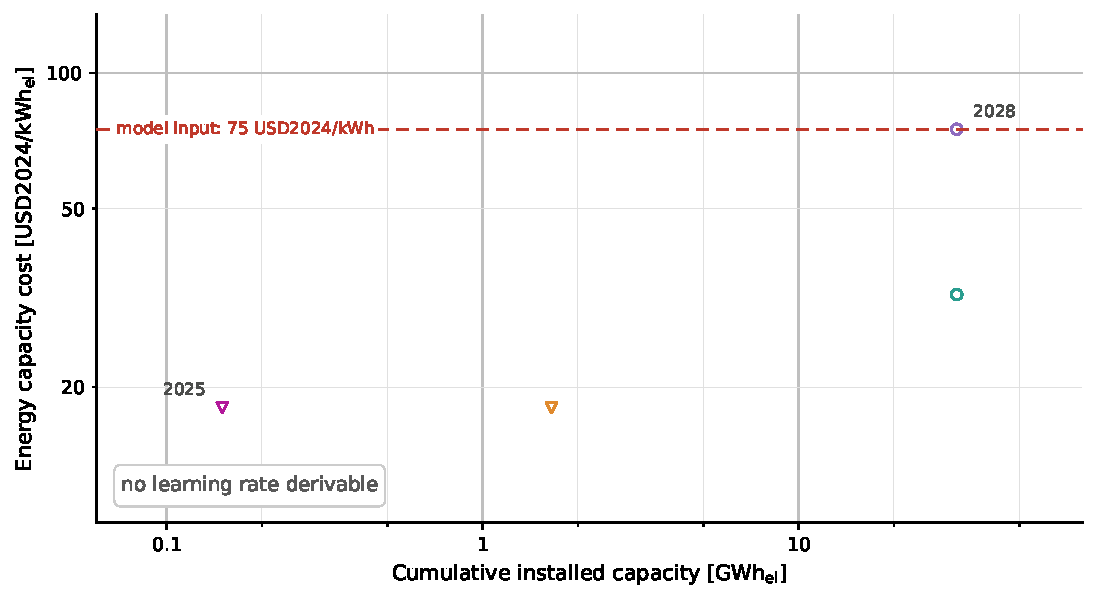
\includegraphics[width=\textwidth]{../../../misc-quarter1/technology-costs/figures/learning/iron-air.pdf}
\caption{
  Iron-air battery cost per kWh against cumulative capacity.
  Triangles: Form's cost target from its modelling recommendations [1] and vendor target [2] \citep{form2023}.
  Circles: Pine Island after incentives [3] \citep{techcrunch2026} and before incentives [4] \citep{weaver2026}.
  Dashed red line: the model input.
}\label{fig:iron-air}
\end{figure}

The learning rate is 15\,\% on the energy part.
There is no cost history yet, so we use a literature value of $15\pm5$\,\% \citep{riepin2025}.
At this rate, reaching Form's target of 15--20~\$/kWh \citep{form2023} takes eight to ten doublings of cumulative capacity.

The efficiency of 0.41 is the product of 0.70 for charging and 0.59 for discharging, and the fixed O\&M is 1\,\% per year of a 35~\$/kWh system, both from Form's modelling recommendations \citep{form2023}.
Existing capacity is Great River Energy's 1.5~MW / 150~MWh pilot in Cambridge, Minnesota; further projects are under construction or planned at Pine Island and in Georgia and Maine.
The lead time is 1.5~years.

\needspace{15\baselineskip}% room for the wrapped icon (it cannot break across pages)
\subsection{Enhanced geothermal, EGS (7,900~\$/kW at Cape Station)}\label{sec:egs}
\techicon{egs}{A drilling rig over two horizontal wells, joined by stimulated fractures in hot rock.}
Enhanced geothermal systems (Figure~\ref{fig:icon-egs}) create a reservoir in hot, dry rock by drilling and hydraulic fracturing, using methods from the oil and gas industry.
This enables heat extraction at places where conventional geothermal would not be viable.
They give firm, carbon-free power, typically through a binary plant (organic Rankine cycle) whose working fluid boils at the comparatively low reservoir temperatures.


EGS cost varies strongly from site to site, so the CAPEX of 7,900~\$/kW is that of one reference site, Fervo's Cape Station in Utah (red circle in Figure~\ref{fig:egs-maps}).
It lies about 15\,\% above Fervo's own estimate of about 7,000~\$/kW for the first phase of Cape Station \citep{fervos1} (Figure~\ref{fig:egs}, right axis).
Our value is per kW of net output, after the parasitic load of wellfield pumps; Fervo does not say which it reports.

In the model, EGS uses supply curves per grid cell, which we build with the cost model of \citet{ricks2025}:
\begin{itemize}[nosep,leftmargin=*]
\item \textbf{Temperature at depth:} inferred from heat conduction from the heat-flow map of \citet{lucazeau2019} for every 0.25$^\circ$ land cell globally.
\item Depth: five candidate depths from 2.5 to 6.5~km; reservoirs below 150\,\textdegree C are not developed.
\item \textbf{Surface plant:} a binary plant whose cost and output follow from the production temperature, after heat loss in the well and a correction for the ambient temperature.
\item \textbf{Net output:} the cost model omits the power demand of the wellfield pumps; to account for this, we subtract 15\,\% of the output, such that all costs are per kW of net output.
\item \textbf{Wellfield:} horizontal wells with 2.3~km laterals and 1.5 producers per injector; drilling cost rises quadratically with depth, plus stimulation, exploration and interest during construction.
\item \textbf{Depth trade-off per cell}: deeper wells cost more, but reach hotter rock, so each well yields more heat and the plant converts it more efficiently.
Each cell takes the depth with the lowest LCOE (7\,\%, 30~years, capacity factor 0.85), a choice among the five candidate depths.
\item \textbf{Potential:} land counts as available with the exclusions the model applies to onshore wind: the land-cover classes allowed for wind \citep{buchhorn2020}, at least 1~km from urban areas, and outside protected areas \citep{sosa2020}.
\end{itemize}

We inherit these cost relations from \citet{ricks2025} who condensed GETEM, the US Department of Energy's Geothermal Electricity Technology Evaluation Model \citep{mines2016}, into simple formulas.
GETEM is a spreadsheet, developed at Idaho National Laboratory, that costs a geothermal project on a component by component basis (exploration, drilling, stimulation, surface plant, O\&M) from the reservoir temperature and depth.
\citet{ricks2025} conduct a fit of cost per depth and updated drilling costs based on the performance of Utah FORGE and Fervo in 2022--2024.

Figure~\ref{fig:egs-maps} shows the geothermal gradient that drives this cost and the resulting CAPEX per cell.
In the large modelled regions (China, the US, Brazil, North-West Europe and India), the cheapest 10~GW cost 4,700--7,600~\$/kW, while the median land cell costs about 16,500~\$/kW.

At Cape Station, the cheapest depth in the model is 5.5~km, deeper than Fervo drills, because the model's temperature map gives only 166\,\textdegree C at 2.5~km.
For a well of Cape's length (2.5~km deep plus a 2.3~km lateral), the model implies 435~\$ per foot drilled, between Fervo's first and latest Cape wells (Figure~\ref{fig:egs}).
As a result, the model does not assume cheaper drilling than has been demonstrated.

\begin{figure}[htbp]\centering
\begin{subfigure}[t]{0.49\textwidth}\centering
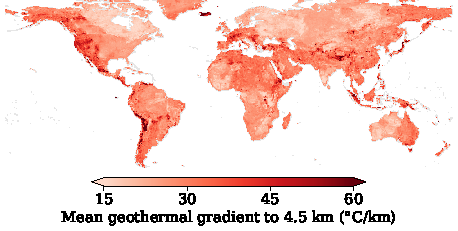
\includegraphics[width=\linewidth]{../../../misc-quarter1/geothermal/figures/egs_doc_gradient.pdf}
\caption{Mean geothermal gradient to 4.5~km}
\end{subfigure}\hfill
\begin{subfigure}[t]{0.49\textwidth}\centering
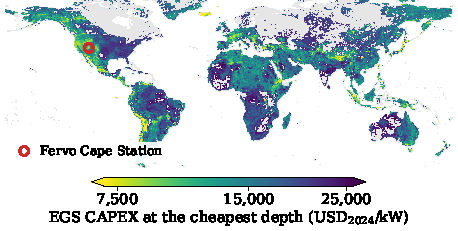
\includegraphics[width=\linewidth]{../../../misc-quarter1/geothermal/figures/egs_doc_capex.pdf}
\caption{EGS CAPEX at the cheapest depth}
\end{subfigure}
\caption{
  Enhanced geothermal on land, 0.25$^\circ$ cells.
  Left: mean temperature gradient from the surface to 4.5~km, from heat conduction on the heat-flow map of \citet{lucazeau2019}.
  Right: CAPEX per kW of net output at each cell's cheapest depth from the cost model of \citet{ricks2025}, 2025 baseline without learning; grey: no reservoir of at least 150\,\textdegree C down to 6.5~km.
  Red circle: Fervo Cape Station, the reference site of Table~\ref{tab:costs} and Figure~\ref{fig:egs}.
  CAPEX colour scale logarithmic.
}
\label{fig:egs-maps}
\end{figure}

\begin{figure}[htbp]\centering
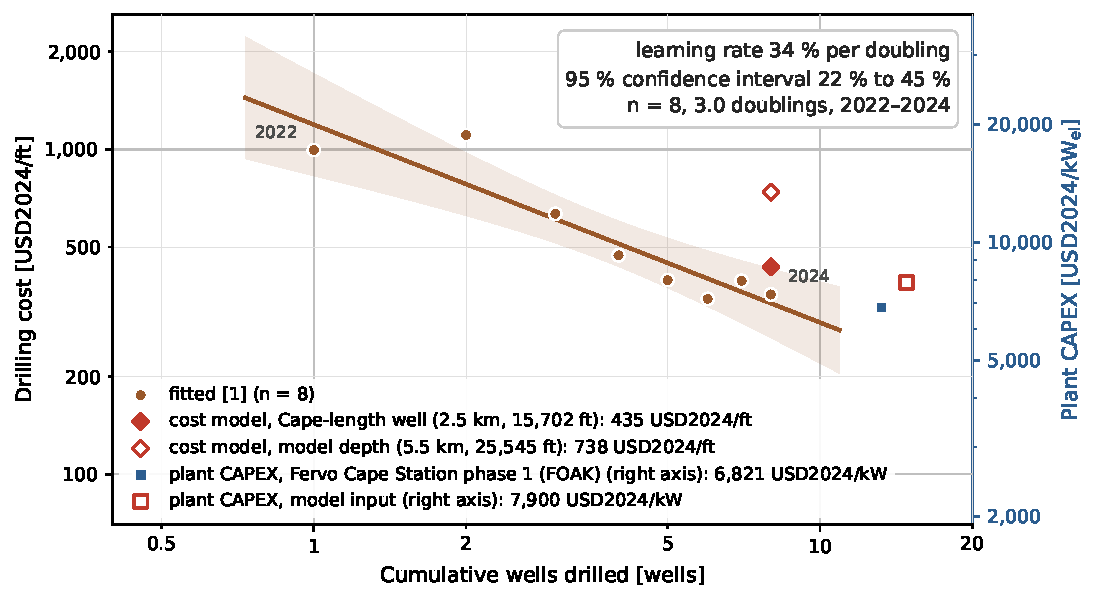
\includegraphics[width=\textwidth]{../../../misc-quarter1/technology-costs/figures/learning/egs.pdf}
\caption{Fervo Cape Station, Utah (red circle in Figure~\ref{fig:egs-maps}): drilling cost per foot of Fervo's EGS wells against cumulative wells drilled, and whole-plant CAPEX.
The first two wells are Fervo's Project Red in Nevada, all others are at Cape Station.
Source: [1] El-Sadi et al.\ (2024), as tabulated by \citet{akindipe2025}.
Red diamonds: the cost model of \citet{ricks2025} at the Cape Station cell, for a well of Cape's length (filled) and at the model's cheapest depth (hollow), drawn at Fervo's eighth well.
Squares, right axis: whole-plant CAPEX, Fervo's estimate for Cape Station phase~1 \citep{fervos1} (filled) and the model input of Table~\ref{tab:costs} (hollow), drawn at the right, without meaning on the $x$-axis.}\label{fig:egs}
\end{figure}

Regarding learning, we inherit the assumptions of \citet{ricks2025}, which split cost reductions into the wellfield and the surface plant.
Wellfield costs (drilling and stimulation) fall by 15\,\% per doubling, starting from 500~MW of EGS assumed by 2030, and surface binary plants by 10\,\% per doubling, starting from about 4~GW of binary capacity worldwide.
We do not carry their additional R\&D-driven decline of 0.5\,\% per year.
Fervo's first eight wells show faster drilling learning of 34\,\% per doubling (Figure~\ref{fig:egs}), but over only three doublings.

The fixed O\&M of 164~\$/kW/yr is the cost model's value at Cape Station, and the lifetime is 30~years.
The capacity factor of 0.85 lies between the 0.8 that NREL's ATB uses for binary plants and 0.9 \citep{atb2024}.
Existing capacity is Fervo's Project Red; the pipeline is Fervo's Cape Station (500~MW by 2028).
The lead time is 3~years.

% Conventional hydrothermal geothermal is a separate, mature row (Section~\ref{sec:geothermal}).

\needspace{15\baselineskip}% room for the wrapped icon (it cannot break across pages)
\subsection{Solid oxide fuel cell on gas (4,100~\$/kW; with carbon capture 4,740~\$/kW)}\label{sec:sofc}
\techicon{sofc}{A solid oxide fuel cell stack: ceramic cells between interconnects; gas and air in, exhaust out.}
A solid oxide fuel cell (SOFC; Figure~\ref{fig:icon-sofc}) turns natural gas into electricity electrochemically, at 59\,\% efficiency, and operates as baseload because it is not suited for ramping.
Its exhaust is mostly CO$_2$ and water, so capture needs no solvent and is cheaper than after a turbine.
Table~\ref{tab:costs} therefore carries the fuel cell without and with capture; only the latter fits a (near-)carbon-neutral system.


Without capture, the CAPEX of 4,100~\$/kW is Bloom Energy's average price per kW but includes a margin \citep{bloom10k}; the fitted product cost at today's 1.4~GW plus installation would be 2,495~\$/kW.

The additional cost for carbon capture have to be estimated.
We here infer them from hypothetical 650~MW plants built from SOFC stacks by NETL \citep{netl2022}.
There, capture adds 640~\$/kW (as the difference between a plant with and without CC 1,627 and 1,116~\$/kW) in 2018 dollars .
The value 640~\$/kW results from the economies of scale of a large 650 MW plant, and is likely less what CC would cost for a smaller Bloom plant.

The learning rate is 30\,\%, fitted to Bloom's product cost (Figure~\ref{fig:sofc}) and extrapolated to the CC component; it rests on one vendor's record and is high compared with similar technologies.
At this rate, the plant with capture reaches the cost of NETL's mature plant \citep{netl2022}, about 2,030~\$/kW in 2024 dollars, after about 2.4 doublings, near 7~GW of cumulative capacity.

\begin{figure}[htbp]\centering
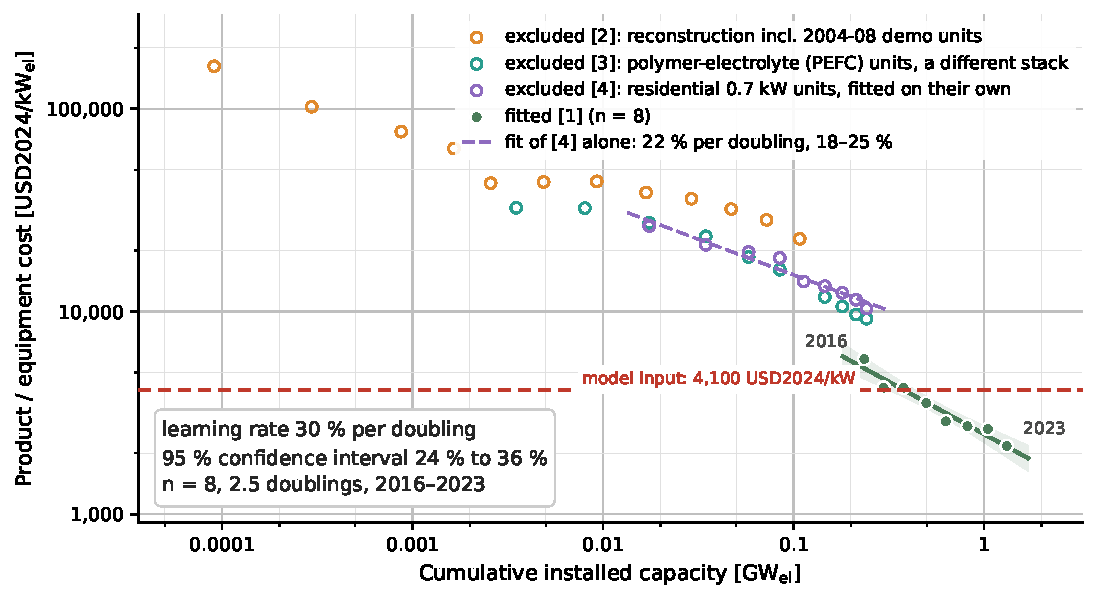
\includegraphics[width=\textwidth]{../../../misc-quarter1/technology-costs/figures/learning/sofc.pdf}
\caption{Fuel cell cost per kW against cumulative capacity.
Filled and fitted: Bloom Energy product cost [1] \citep{bloom10k}.
Hollow, for context: residential ENE-FARM units in Japan, as reconstructed by \citet{schmidt2018} [2] and from the official shipment statistics \citep{ace2025} for polymer-electrolyte [3] and solid oxide [4] units.
Dashed red line: the model input.}\label{fig:sofc}
\end{figure}

The fixed O\&M is 5\,\% of CAPEX per year, the DEA's figure for fuel cells \citep{dea}.
Capture lowers the efficiency to 0.55, removes 97.8\,\% of the CO$_2$ \citep{netl2022}.
We further assume this adds 4.5~\$/MWh for CO$_2$ transport and storage at NETL's 10~\$/t .
Existing capacity approximates Bloom's cumulative deployment, with no pipeline.
The lead time is 1~year \citep{eia2023}.

The gas price is the default of 20~\$/MWh\textsubscript{th} (Section~\ref{sec:CCGT}); where imported LNG sets the price, as in Europe, the model should add the cost of liquefaction.

The stacks last about five years and must be replaced, which the cost assumptions do not yet reflect.

\needspace{15\baselineskip}% room for the wrapped icon (it cannot break across pages)
\subsection{Vanadium flow battery, 8~h (193.1~\$/kW + 398.5~\$/kWh)}\label{sec:vrfb}
\techicon{vrfb}{Two electrolyte tanks feeding a cell stack through pumps.}
Not part of the default pool of advanced technologies, only listed here for transparency about its exclusion.

A vanadium flow battery (Figure~\ref{fig:icon-vrfb}) stores energy in tanks of liquid electrolyte, so power and energy can be sized separately.
It suits durations of roughly 4--12~hours, which puts it between Li-ion and multi-day storage such as iron-air.


The CAPEX of 193.1~\$/kW for the power part and 398.5~\$/kWh for the energy part, at 8~hours, is the figure of technology-data \citep{technologydata}.

We leave the technology out because its cost floor is likely to lose out to Li-ion.
That floor is set by the vanadium in the electrolyte:
one kWh needs 5.6~kg of vanadium pentoxide in theory and about 8~kg at today's utilisation.
At the 2024 Chinese price, this implies costs of 67--96~\$/kWh \citep{usgs2025} before tanks, pumps and stacks are added.
With the numbers of Table~\ref{tab:costs}, an 8-hour Li-ion system already costs about 315~\$/kWh against 423~\$/kWh for the flow battery, and Li-ion is still reducing in cost.
Flow batteries would therefore lose in the 4--12-hour range to Li-ion, while iron-air serves longer durations at lower cost.

The learning rate is 22\,\% on the energy part, fitted to the cost series of \citet{schmidt2018} extended with recent Chinese projects (Figure~\ref{fig:vrfb}); Schmidt et al.\ themselves published 13~$\pm$~3\,\%.

\begin{figure}[htbp]\centering
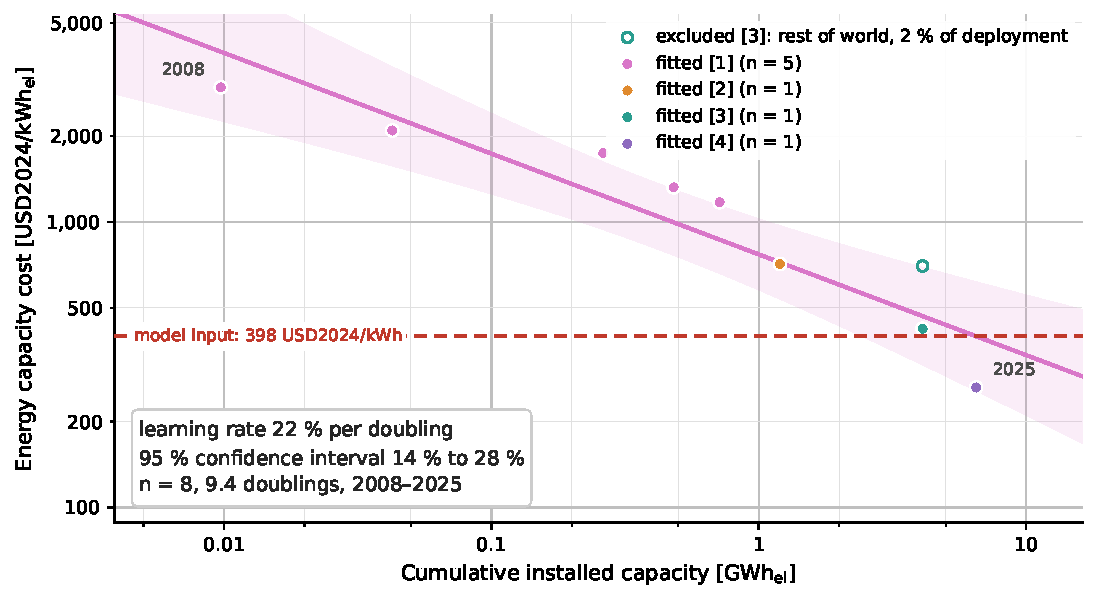
\includegraphics[width=\textwidth]{../../../misc-quarter1/technology-costs/figures/learning/vrfb.pdf}
\caption{Vanadium flow battery cost per kWh of storage against cumulative capacity.
Sources: [1] \citet{schmidt2018}; [2] Dalian Rongke, 100~MW / 400~MWh \citep{pvmag2022}; [3] installed system cost in China (filled) and in the rest of the world (hollow, 2\,\% of deployment, not fitted) from BNEF's 2024 survey \citep{esn2025}; [4] Rongke, 200~MW / 1~GWh in Xinjiang, supplier price \citep{projectblue2025}.
Cumulative capacity after 2017 counts Chinese additions only.
Dashed red line: the model input.}\label{fig:vrfb}
\end{figure}

The fixed O\&M of 4.7~\$/kW/yr plus 0.93~\$/kWh/yr over 8~hours and the 12-year lifetime come from technology-data \citep{technologydata}.
The table's efficiency of 0.806 is the value of technology-data \citep{technologydata} for one direction (charging or discharging); the round trip is 0.65.
Existing capacity is about 1~GW: roughly 4~GWh of flow batteries were installed by the end of 2024, mostly in China, at a typical duration of 4~hours (our compilation of \citet{schmidt2018} and recent project data).
The lead time is 1~year.

\needspace{15\baselineskip}% room for the wrapped icon (it cannot break across pages)
\subsection{CO$_2$ battery, 10~h (2,449~\$/kW + 244.9~\$/kWh)}\label{sec:co2-battery}
\techicon{co2-battery}{An inflatable dome holding CO$_2$ gas, beside vessels of liquid CO$_2$ and the compressor-turbine.}
Not part of the default pool of advanced technologies, only listed here for transparency about its exclusion.

Energy Dome's (the company pushing this technology forward) CO$_2$ battery (Figure~\ref{fig:icon-co2-battery}) stores energy by compressing CO$_2$ gas into a liquid and releases it through a turbine.
It is built from conventional compressors, turbines and tanks and suits durations of around 10~hours.
Its landmark is a large white inflatable dome that holds the CO$_2$ as gas at atmospheric pressure while the battery is empty; a 20~MW / 200~MWh plant covers about 5~hectares, most of it dome \citep{utilitydive2024}.

The CAPEX of 2,449~\$/kW plus 244.9~\$/kWh at 10~hours follows Energy Dome's disclosed price of about 220~EUR\textsubscript{2023}/kWh for the whole system, quoted for its first full-scale plant including engineering, construction and margin \citep{esn2023}.
Alliant's US plant of the same size is budgeted at 60--90~million~USD, or 300--450~\$/kWh \citep{utilitydive2024}.

We leave the technology out because it is too similar to iron-air to be included as well.
Both are long-duration storage built from cheap, abundant materials, and both would fill the same gap beyond Li-ion.
Iron-air is the stronger candidate for this role: its energy part costs less than a third (75 against 245~\$/kWh), and it has a large procured project at Pine Island.
The CO$_2$ battery's higher round-trip efficiency (0.75 against 0.41) suits daily cycling better, so it may be assessed as a sensitivity.

The learning rate is 5\,\% on the energy part; there is no cost history.
It is an analogy to mature mechanical storage: the plant consists of conventional compressors, turbines and tanks, whose costs no longer fall much, and pumped hydro, the closest analogue, shows no learning ($-1 \pm 8$\,\%, \citealp{schmidt2018}).

The round-trip efficiency is 0.75 \citep{esn2023}, 0.73--0.75 according to Alliant \citep{utilitydive2024}, and the lifetime 30~years \citep{energydome}.
No fixed O\&M has been published, so the cell is blank.
Existing capacity is the 2.5~MW / 4~MWh demonstrator at Ottana, Sardinia, in trials since 2022 \citep{mittr2022}; the pipeline is a 20~MW / 200~MWh plant at the same site and Alliant Energy's plant of the same size in Columbia, Wisconsin \citep{utilitydive2024}.
The lead time of 2~years is our assumption for a plant of conventional components; the Sardinian plant has slipped from completion in 2024 \citep{utilitydive2024} to 2025 \citep{engie2024}, so it may be longer.


\section{Mature technologies}
We apply no endogenous technology learning to these technologies; instead, their costs follow the fixed path projected by the Danish Energy Agency (DEA) catalogue \citep{dea}.
Unless stated otherwise, their 2025 costs come from PyPSA/technology-data v0.15.0 \citep{technologydata}, which carries the DEA figures, converted to USD\textsubscript{2024}.
Existing capacities are Ember's 2024 figures \citep{ember2025} unless stated otherwise.
The water-cooled nuclear reactors are the exception: their costs come from our own project data and stay constant.

\subsection{Solar PV, utility scale (655~\$/kW)}\label{sec:solar-utility}
Utility-scale solar PV has seen extensive learning, and is the cheapest clean source of electricity in sunny regions.

The CAPEX of 655~\$/kW is the 2025 value of the Danish Energy Agency (DEA) catalogue \citep{dea} as carried by technology-data \citep{technologydata}.
We apply an exogenous cost path from the DEA projections \citep{dea}.
For reference, installed costs have fallen by about a third with each doubling of cumulative capacity (Figure~\ref{fig:solar}).

\begin{figure}[htbp]\centering
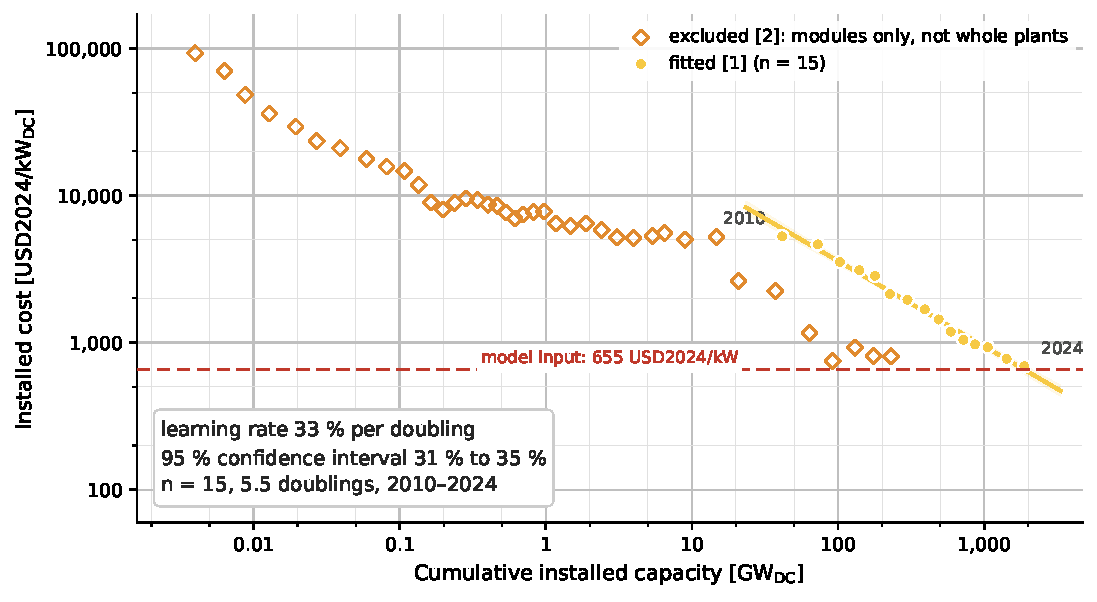
\includegraphics[width=\textwidth]{../../../misc-quarter1/technology-costs/figures/learning/solar-utility.pdf}
\caption{Installed cost of utility-scale PV against cumulative capacity.
Sources: [1] \citet{irena2025}, fitted; [2] module prices of \citet{schmidt2018}, for context.
Dashed red line: the model input.}\label{fig:solar}
\end{figure}

The fixed O\&M and the 37.5-year lifetime come from technology-data \citep{technologydata}, existing capacity from Ember \citep{ember2025}.
The capacity factor of 0.18 in Table~\ref{tab:costs} is a reference value, while the model uses hourly weather-based profiles for every region (Figure~\ref{fig:solar-maps}).

\begin{figure}[htbp]\centering
\begin{subfigure}[t]{0.49\textwidth}\centering
\includegraphics[width=\linewidth]{../build/figures/solar-utility_cf.pdf}
\caption{Annual mean capacity factor}
\end{subfigure}\hfill
\begin{subfigure}[t]{0.49\textwidth}\centering
\includegraphics[width=\linewidth]{../build/figures/solar-utility_lcoe.pdf}
\caption{Levelised cost of electricity}
\end{subfigure}
\caption{Utility-scale solar PV on land, 0.5$^\circ$ cells.
Left: annual mean capacity factor from ERA5 weather of 2011 \citep{hersbach2020}, as converted by \href{https://model.energy}{model.energy} \citep{modelenergy}.
Right: the levelised cost this implies with the costs of Table~\ref{tab:costs} at a 7\,\% real discount rate; colour scale logarithmic.}\label{fig:solar-maps}
\end{figure}

Regional differences in the cost of capital could be considered: in low- and middle-income countries, high financing costs add on average 26~\$/MWh to the levelised cost of solar \citep{hatton2026}.

\subsection{Onshore wind (1,584~\$/kW)}\label{sec:onwind}
Onshore wind can provide low-cost clean electricity and complement solar's intermittency or low regional suitability.

The CAPEX of 1,584~\$/kW is the 2025 value of the DEA catalogue \citep{dea} as carried by technology-data \citep{technologydata}.
It lies well above the global average of 1,041~\$/kW that IRENA reports for 2024 (Figure~\ref{fig:onwind}).

The global average is dominated by China, which installs most new wind at much lower turbine and construction costs (856~\$/kW in 2024), while the DEA describes Danish projects.
The rest of the world is closer to Europe than to China \citep[Table~2.1]{irena2025}: India builds at 1,110~\$/kW, but most other regions at 1,240--1,490~\$/kW (Africa, Oceania, Brazil, the rest of the Americas), the US at 1,568 and Europe at 1,659~\$/kW, and the rest of Asia, including Japan and Korea, at 1,912~\$/kW.
Our value thus fits most regions outside China and India.
DEA turbines also have large rotors for their rating, which costs more per kW but yields a higher capacity factor.
Lower regional CAPEX may be needed for China and India.

\begin{figure}[htbp]\centering
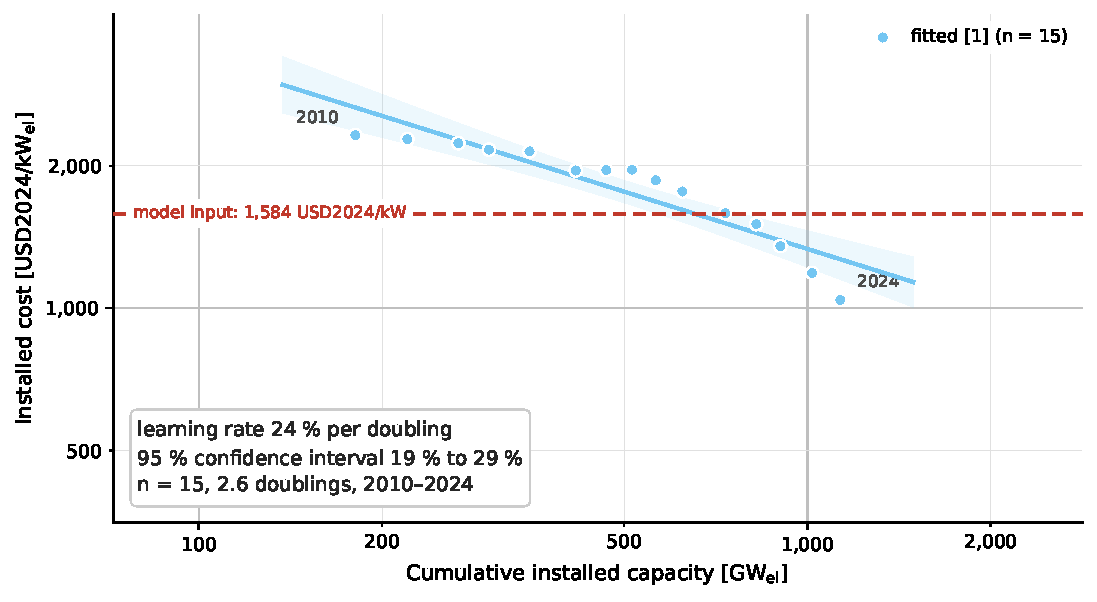
\includegraphics[width=\textwidth]{../../../misc-quarter1/technology-costs/figures/learning/onwind.pdf}
\caption{Installed cost of onshore wind against cumulative capacity.
Source: [1] \citet{irena2025}, fitted.
Dashed red line: the model input.}\label{fig:onwind}
\end{figure}

We apply an exogenous cost path from the DEA projections \citep{dea}.

O\&M and the 28.5-year lifetime come from technology-data \citep{technologydata}.
Existing capacity is Ember's 2024 wind total minus the offshore fleet reported by the Global Wind Energy Council \citep{gwec2025}.

Wind resources vary even more than solar radiation (Figure~\ref{fig:onwind-maps}).
The best sites, in Patagonia, the British Isles, the US and southern Australia, reach capacity factors of 0.4--0.6 and a levelised cost of 30--45~\$/MWh.

\begin{figure}[htbp]\centering
\begin{subfigure}[t]{0.49\textwidth}\centering
\includegraphics[width=\linewidth]{../build/figures/onwind_cf.pdf}
\caption{Annual mean capacity factor}
\end{subfigure}\hfill
\begin{subfigure}[t]{0.49\textwidth}\centering
\includegraphics[width=\linewidth]{../build/figures/onwind_lcoe.pdf}
\caption{Levelised cost of electricity}
\end{subfigure}
\caption{Onshore wind, 0.5$^\circ$ cells.
Left: annual mean capacity factor from ERA5 weather of 2011 \citep{hersbach2020}, as converted by \href{https://model.energy}{model.energy} \citep{modelenergy}.
Right: the resulting levelised cost with the costs of Table~\ref{tab:costs} at a 7\,\% real discount rate.}\label{fig:onwind-maps}
\end{figure}

Regional differences in the cost of capital could be considered: in low- and middle-income countries, high financing costs add on average 24~\$/MWh to the levelised cost of onshore wind \citep{hatton2026}.

\subsection{Offshore wind (2,449~\$/kW)}\label{sec:offwind}
Offshore wind turbines reach higher capacity factors, because winds at sea are stronger and steadier.
They cost more to build, but produce more per kW and avoid land-use conflicts.

The CAPEX of 2,449~\$/kW is the 2025 value of the DEA catalogue \citep{dea} as carried by technology-data \citep{technologydata}.

We apply an exogenous cost path from the DEA projections \citep{dea}.

O\&M and the 30-year lifetime come from technology-data \citep{technologydata}; the existing capacity of about 83~GW at the end of 2024 from the Global Wind Energy Council \citep{gwec2025}.
The lead time is 4~years.

Like wind on land, the offshore resource varies strongly (Figure~\ref{fig:offwind-maps}).
The best shallow seas, the North Sea, the Taiwan Strait and the shelf off Patagonia, reach capacity factors around 0.6 and a levelised cost below 50~\$/MWh; the Baltic and the Bass Strait follow closely, while the tropical shelves of South-East Asia have little wind.
These capacity factors are an upper bound: they come from an onshore turbine model and leave out the wake losses within large offshore farms, so they lie above the 0.45 of Table~\ref{tab:costs}.

\begin{figure}[htbp]\centering
\begin{subfigure}[t]{\textwidth}\centering
\includegraphics[width=\linewidth]{../build/figures/offwind_cf.pdf}
\caption{Annual mean capacity factor}
\end{subfigure}

\medskip
\begin{subfigure}[t]{\textwidth}\centering
\includegraphics[width=\linewidth]{../build/figures/offwind_lcoe.pdf}
\caption{Levelised cost of electricity}
\end{subfigure}
\caption{Offshore wind on shallow sea, 0.5$^\circ$ cells with at least a quarter of their area 0--50~m deep (the model's depth limit; bathymetry of \citealp{gebco2025}), south of the Arctic circle; cells are drawn enlarged, about 2.5 times their width, so the narrow coastal strips stay visible.
Top: annual mean capacity factor from ERA5 weather of 2011 \citep{hersbach2020}, as converted by \href{https://model.energy}{model.energy} \citep{modelenergy} with its onshore turbine, as a proxy.
Bottom: the resulting levelised cost with the costs of Table~\ref{tab:costs} at a 7\,\% real discount rate; colour scale logarithmic.}\label{fig:offwind-maps}
\end{figure}

\subsection{Hydro, reservoir (3,180~\$/kW)}\label{sec:hydro}
Reservoir hydro stores water behind dams and releases it when power is needed.
It is clean, flexible and dispatchable, and can complement intermittent renewables, a dynamic that the hydro-rich archetype should capture.

The CAPEX of 3,180~\$/kW is the figure of technology-data \citep{technologydata}.
However, reservoir hydro relies on suitable natural topography, and the best resources have largely been exploited.
Therefore, the model fixes the existing fleet and allows new reservoirs only in rare cases.

We apply no learning.

The fixed O\&M and the 80-year lifetime come from technology-data \citep{technologydata}; the existing capacity from Ember includes run-of-river plants.

\subsection{Hydro, run-of-river (4,770~\$/kW)}\label{sec:ror}
Run-of-river plants have no large reservoir and produce whatever the river carries, so their output follows the seasons and cannot be shifted.

The CAPEX of 4,770~\$/kW is the figure of technology-data \citep{technologydata}, kept for completeness; as for reservoir hydro, we fix the existing fleet.

We apply no learning.

The fixed O\&M and the 80-year lifetime come from technology-data \citep{technologydata}; existing capacity is counted under reservoir hydro.

\subsection{Geothermal, hydrothermal (4,887~\$/kW)}\label{sec:geothermal}
Conventional geothermal plants tap rare natural reservoirs of hot water or steam.
They give firm, carbon-free power, but only where such reservoirs exist, mostly along volcanic belts.

The CAPEX of 4,887~\$/kW is NREL's ATB 2024 cost for flash plants \citep{atb2024}; binary plants for cooler resources cost 6,420~\$/kW.

We apply no learning, and by default the model builds no new conventional geothermal, because the remaining reservoirs are few, site-specific and slow to develop.

The fixed O\&M, the capacity factor of 0.9 and the 30-year lifetime come from the same ATB entry, NREL's representative flash plant.
% Existing capacity (IRENA) and the pipeline (GEM) come from our geothermal dataset in \texttt{misc-quarter1/geothermal}, which also estimates the potential per country that caps new building.
Existing capacity is IRENA's installed 15.6~GW \citep{irenastats}.

\subsection{Biomass (3,249~\$/kW)}\label{sec:biomass}
Biomass plants burn solid fuel such as wood chips or agricultural residues in a steam cycle.
They are dispatchable, but limited by the supply of sustainable fuel.
Moreover, biomass is worth more for its carbon than for its energy: captured for negative emissions or used as feedstock for e-fuels \citep{millinger2025}.
In the same study, bioelectricity mainly helps reliability as dispatchable backup for about 1\,\% of generation.

The CAPEX of 3,249~\$/kW is the figure of technology-data \citep{technologydata}.

We apply no learning.

O\&M and the 30-year lifetime come from technology-data \citep{technologydata}; existing capacity from Ember \citep{ember2025}.
The fuel price of 19.1~\$/MWh\textsubscript{th} is technology-data's entry for solid biomass, forest-residue wood chips from the JRC ENSPRESO database; traded chips and pellets cost more.
The efficiency of 0.30 is the net electrical efficiency of the DEA's large straw-fired plant \citep{dea}; technology-data's older entry of 0.468 is too high for a dedicated biomass plant.

\subsection{Nuclear LWR, China and India (3,150~\$/kW)}\label{sec:nuclear-lwr-cnin}

Recent project data show that China and India build light- and heavy-water reactors at lower cost than other countries, and the West in particular (Figure~\ref{fig:nuclear-strip}), so we give them their own cost bin.
The usual explanation is that both countries build in series, with dedicated crews moving from site to site.

Audited final costs are rarely published there, so ex-post construction costs are largely unavailable.
We therefore scale the available ex-ante figures by 1.27, the median ratio of final (or latest) to initial estimate over all projects in our dataset that report both.

\begin{figure}[htbp]\centering
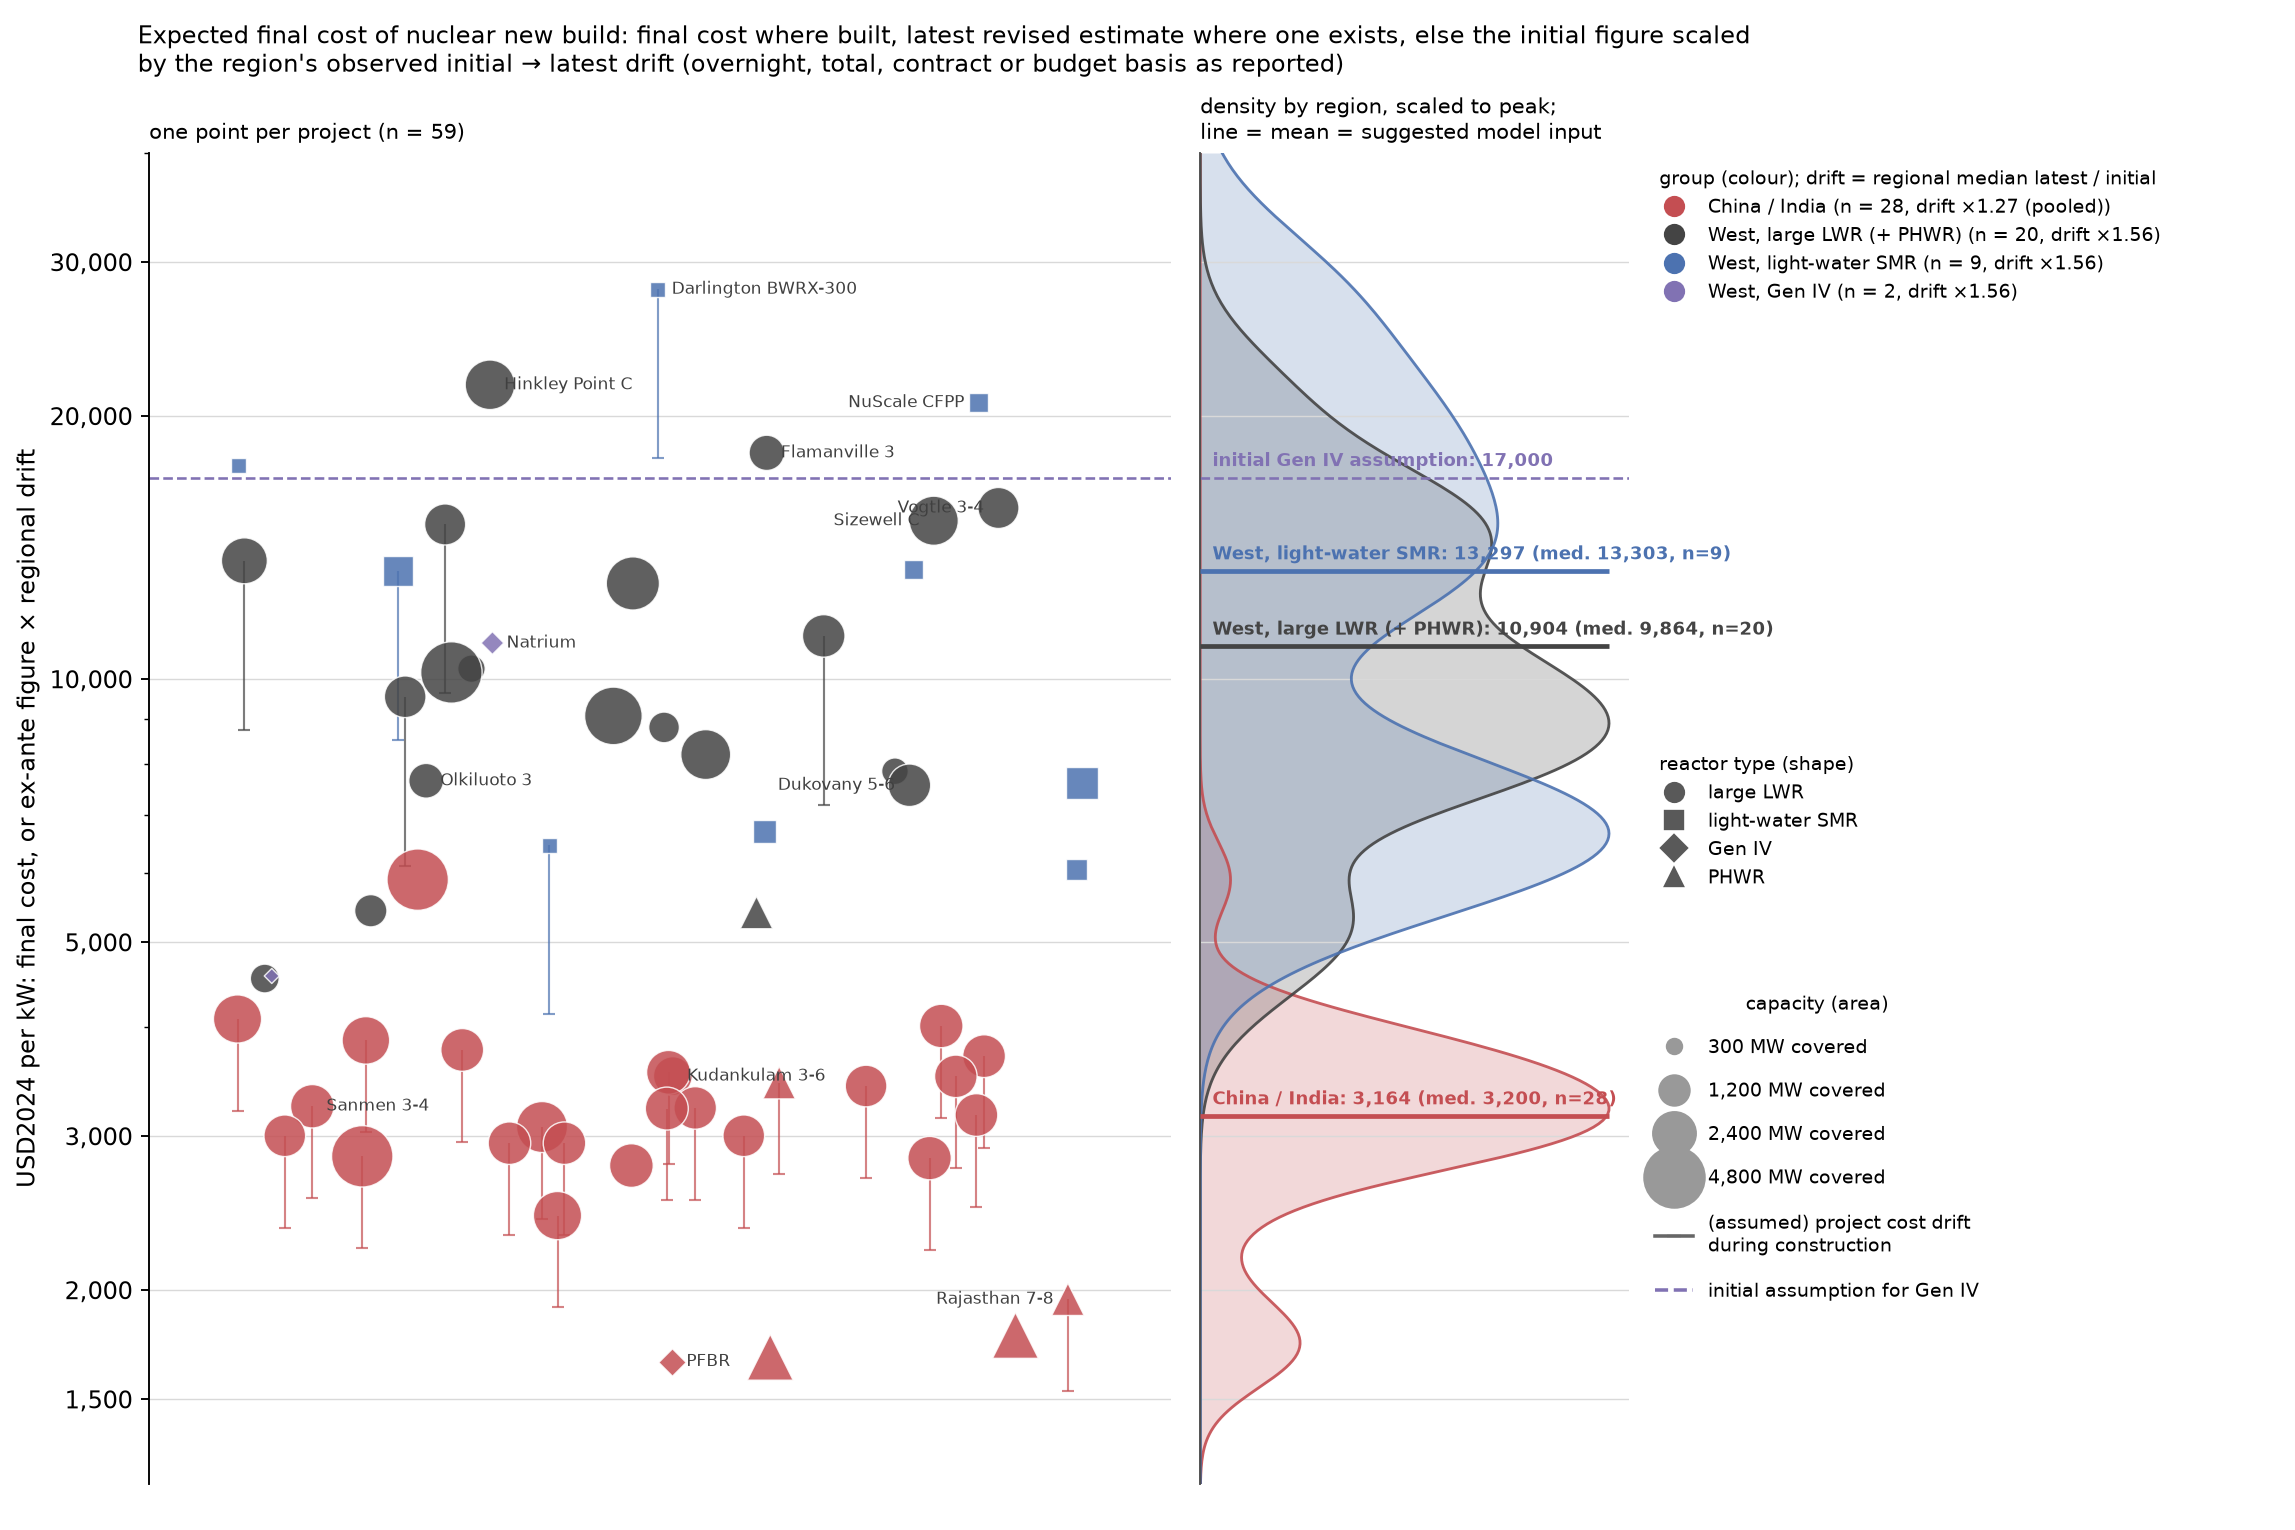
\includegraphics[width=\textwidth]{../../../misc-quarter1/nuclear-projects/figures/nuclear_cost_strip.png}
\caption{
  Expected final cost per kW of nuclear projects with a published figure, by region and reactor type:
  final cost where built, latest estimate where available, otherwise the initial estimate is scaled by the observed regional drift.
  One point per project; vertical lines lead from the initial estimate to the expected final cost.
  The points are 59 projects compiled from public sources, each with its source in \texttt{misc-quarter1/nuclear-projects/data/project\_costs.csv}; unit data from the GEM tracker \citep{gem2026}.
}
\label{fig:nuclear-strip}
\end{figure}

Based on these projects, we use 3,150~\$/kW (median 3,200; Figure~\ref{fig:nuclear-strip}).
For simplicity, large reactors and SMRs share the bin.

The learning rate is zero.
Both countries build reactors in series and their costs have been flat since 2010, so there is no evidence for further learning.

O\&M cost, efficiency and the 60-year lifetime come from technology-data's nuclear entry \citep{technologydata}.
The fuel price of 2~\$/MWh\textsubscript{th}, about 6~\$ per MWh of electricity, follows from US plants, where fuel makes up 15--20\,\% of a generating cost of about 31~\$/MWh \citep{doe2024nuclear}; technology-data's 8.2~\$/MWh\textsubscript{th} is four times higher.
The lead time of 6~years is China's median build time \citep{gem2026}.

Without a build limit, the model would build excessive nuclear capacity in China and India.
Construction currently starts at about 10~GW/yr in China (11~GW in 2025) and 2~GW/yr in India \citep{gem2026};
we carry these into the model, and show for representation their sum 12~GW/yr in this document's Table~\ref{tab:deployment}.

\subsection{Nuclear LWR, rest of world (11,000~\$/kW)}\label{sec:nuclear-lwr-row}

This bin covers new water-cooled reactors built outside China and India.
Such projects have become more expensive over the past half-century \citep{eashgates2020}.

The CAPEX of 11,000~\$/kW is the average of Western nuclear projects of the last decades (Figure~\ref{fig:nuclear-strip}).
It is slightly below the 11,900~\$/kW of technology-data \citep{technologydata}, the usual source for European studies.
The most recent Western reactors, Vogtle, Flamanville and Hinkley Point~C, came out higher still at 12,000--22,000~\$/kW.
Either way, this cost is too high for the model to pick up water-cooled nuclear in the West, even in a carbon-neutral setting.

Some countries have built nuclear plants at reliably lower cost than the West, notably South Korea \citep{lovering2016} and Russia.
We neglect this nuance because neither lies within our regions of focus.

The learning rate is zero.
The historical record for large light-water reactors ranges from negative to 6\,\% \citep{rubin2015,eashgates2020}.

All other parameters are those of the China--India bin; the lead time is 10~years.
The build limit of 7~GW/yr is the most construction started outside China and India in any year of the last decade (2024) \citep{gem2026}; at this CAPEX, the model is unlikely to reach it.

\subsection{Gas combined cycle, CCGT (2,500~\$/kW)}\label{sec:CCGT}
A combined-cycle gas turbine is the most efficient fossil power plant and today's main source of flexible baseload in many regions.

The CAPEX of 2,500~\$/kW reflects recent new-build quotes in the US and Europe.
Since 2024, gas turbine supply has not been able to keep up with demand.
The main suppliers, GE~Vernova, Siemens~Energy and Mitsubishi report order queues to 2029--30, and new US plants are quoted at 2,000--2,500~\$/kW with four- to five-year lead times.

Before the shortage, technology-data \citep{technologydata} carried 1,257~\$/kW, a DEA figure.

We apply no learning.

Efficiency, O\&M and the 25-year lifetime come from technology-data \citep{technologydata}.

The gas price is a global default of 20~\$/MWh\textsubscript{th} (about 5.9~\$/MMBtu), between pipeline gas in North America and imported LNG in Europe and Asia; technology-data's 47.2~\$/MWh\textsubscript{th} \citep{technologydata} is a European value.
For the 2024 calibration, the model uses regional prices instead, e.g.\ 7~\$/MWh\textsubscript{th} in North America and 34~\$/MWh\textsubscript{th} in Europe.
Existing capacity is Ember's 2024 gas total of 2,036~GW \citep{ember2025} minus the open-cycle turbines of the OCGT row, so it also holds the remaining gas steam and engine plants; 1,409~GW of it are combined-cycle plants \citep{gemgogpt}.

The turbine shortage plays in important role in creating a market for long-duration storage and other firm clean power in the first place.

\subsection{Gas open cycle, OCGT (1,300~\$/kW)}\label{sec:OCGT}
An open-cycle gas turbine (OCGT) is cheap to build and starts quickly, so it serves as a peaker for the few hours of highest demand.

The CAPEX of 1,300~\$/kW scales the DEA figure of 654~\$/kW in technology-data \citep{technologydata} by the same factor as the CCGT update, which keeps the DEA's ratio between the two.
The turbine shortage applies here too (Section~\ref{sec:CCGT}).

We apply no learning.

Efficiency, O\&M and the 25-year lifetime come from technology-data \citep{technologydata}; the gas price is the default of 20~\$/MWh\textsubscript{th} (Section~\ref{sec:CCGT}).
Existing capacity is the 356~GW of open-cycle gas turbines operating worldwide \citep{gemgogpt}, which includes some oil-fired units.

\subsection{Li-ion battery, 4~h (316.5~\$/kW + 275.3~\$/kWh)}\label{sec:battery-liion}
Lithium-ion batteries shift power in the short term and so provide intra-day balancing and fast reserves, typically for 2--4~hours.

The CAPEX of 316.5~\$/kW for the inverter and 275.3~\$/kWh for the battery pack is the 2025 DEA figure \citep{dea} as carried by technology-data \citep{technologydata}.

Learning is treated exogenously; the fitted experience rate of 19\,\% on four data points of BloombergNEF's battery cost survey \citep{bnef2025} (Figure~\ref{fig:liion}) is shown for reference only.

\begin{figure}[htbp]\centering
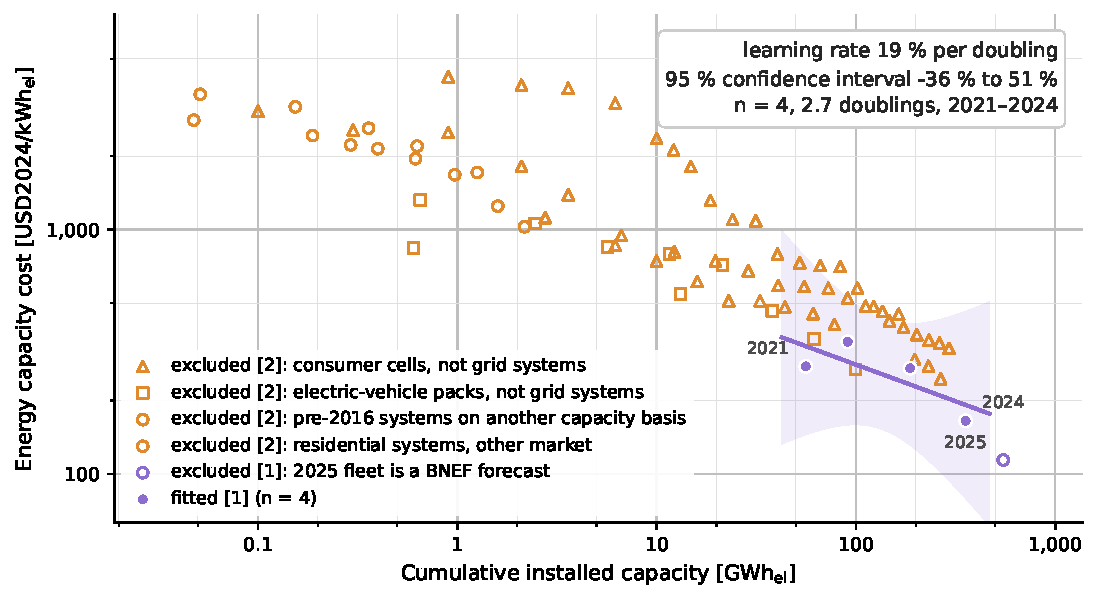
\includegraphics[width=\textwidth]{../../../misc-quarter1/technology-costs/figures/learning/battery-liion.pdf}
\caption{Li-ion energy capacity cost against cumulative capacity.
Sources: [1] turnkey system costs of the BNEF survey \citep{bnef2025}, fitted (the 2025 point is a forecast and excluded); [2] series of \citet{schmidt2018} for cells, electric-vehicle packs and residential systems, for context.
Dashed red line: the model input for the energy part.}\label{fig:liion}
\end{figure}

We set the fixed O\&M to 40~USD\textsubscript{2023}/kW/yr, because technology-data \citep{technologydata} gives it per kWh, which overprices short batteries.
The round-trip efficiency of 0.955 and the 22.5-year lifetime come from technology-data \citep{technologydata}.
Existing capacity is the 124~GW of utility-scale batteries the IEA counts at the end of 2024 \citep{iea2026}, almost all of it lithium-ion.

Sodium-ion batteries are also included under this technology.
They compete in the same role within about 20\,\% of lithium-ion cost, but perform better in the cold, so they need less temperature control in cold climates.
This nuance might be added to the model in appropriate regions.

\subsection{Pumped hydro, 10~h (1,934~\$/kW + 79~\$/kWh)}\label{sec:PHS}
Pumped hydro pumps water uphill and releases it through turbines;
it is the oldest and largest form of grid storage, typically with 6--20~hours of storage.

The CAPEX of 1,934~\$/kW plus 79~\$/kWh at 10~hours is the figure of technology-data \citep{technologydata}, kept for completeness, since the existing fleet is fixed.

We apply no learning.

The fixed O\&M of 19.2~\$/kW/yr plus 0.34~\$/kWh/yr over 10~hours and the 60-year lifetime come from technology-data \citep{technologydata}.
The table's efficiency of 0.894 is the per-direction value of technology-data \citep{technologydata} (pumping or generating); the round trip is 0.80.
Existing capacity is about 180~GW (IHA World Hydropower Outlook).


\section{Considered and dropped}
\paragraph{Allam-cycle gas with CCS} 
The solid oxide fuel cell takes the role of low-carbon gas baseload.

\paragraph{Hydrogen chain (electrolysis, storage in tanks or caverns, fuel cells)}
Dropped because it depends too much on location (industrial demand, salt caverns) to be represented in archetypes.
Potentially added at a later point once a basic version of the project is standing.

\paragraph{Closed-loop geothermal} 
Dropped, because enhanced geothermal already represents the next generation of geothermal power.
There is one commercial project (Eavor in Geretsried, Germany), the DOE Liftoff report puts today's cost at about 34,000~\$/kW, and there is no basis for a learning rate.

\paragraph{Fusion}
No cost estimate can be made yet.

\paragraph{Direct air capture and other CO$_2$ removal}
Represented as a cost cut-off of 300--600~EUR/tCO$_2$, not included as a technology.


\printbibliography
\end{document}
